\chapter{Oprogramowanie }

Zadaniem opracowanego oprogramowania jest:
\begin{enumerate}
    \item sterowanie przełączaniem urządzeń docelowych i jego sygnalizacją
    \item implementacja komunikacji poprzez USB lub UART
    \item resetowanie urządzeń docelowych
\end{enumerate}

\section {Oprogramowanie układowe multipleksera SWD}
Kod został napisany w języku C.
Składa się z kilku modułów:
\begin{enumerate}
    \item sterownik USB - moduł ten został dostarczony w większości przez producenta. Odpowiada za komunikację zgodnie z protokołem USB-CDC. Dzięki niemu multiplekser zgłasza się do urządzenia nadrzędnego jako wirtualny port szeregowy. Dodatkowo zaimplementowano w nim bufor kołowy. Dzięki temu uzyskano prosty w obsłudze interfejs komunikacyjny o charakterze strumienia. Z racji pakietowej transmisji protokołu USB, dla wysyłania ciągu znaków w jednym pakiecie, wymagane było umieszczenie procesu w tle, który dopiero po otrzymaniu znacznika końca pakietu ładował dane do bufora kołowego. Dla prostoty i z racji małej ilości danych wysyłanych przez multiplekser SWD, każdy znak wysyłany w stronę komputera jest wysyłany w osobnym pakiecie.
    \item sterownik interfejsu UART - oparty częściowo na warstwie abstrakcji sprzętowej dostarczonej przez producenta. Dodano obsługę bufora kołowego. Obsługa interfejsu UART oparta jest na przerwaniach (przerwanie niepustego bufora wejściowego oraz przerwanie pustego bufora wyjściowego). Urządzenie wykorzystuje to samo API (Application Programming Interface) co wirtualny port szeregowy USB opisany wyżej.
    \item sterownik przełączników oraz wskaźników urządzeń - Ta część oprogramowania skupia się na ustawieniu wyjść za pomocą sterownika GPIO tak, aby linie sygnałowe z programatora zostały przekierowane na odpowiednie urządzenie. Dodatkowo wybrane urządzenie wskazywane jest poprzez diody umieszczone koło gniazd prowadzących do urządzeń docelowych.
    \item interfejs wiersza poleceń (Command Line Interface - CLI) - nasłuchuje znaków odebranych jednocześnie z USB jak i UART (połączone strumienie wejściowe) i po znalezieniu znaku nowej linii przeszukuje ciąg znaków pod kątem znaku odstępu. Znaki przed nim to nazwa komendy, a znaki do nowej linii to argument. Proces CLI działający w tle przeszukuje listę jednokierunkową komend i jeśli znajdzie tę komendę - wykonuje ją przekazując jej argument. Jeśli komenda nie została znaleziona - zwraca informację o błędzie na połączony strumień wyjścia, który rozdziela się na USB i UART.
    \item sterownik przycisków - korzysta ze sterownika GPIO i NVIC dostarczonych przez producenta. czeka na przerwanie pochodzące od przycisków i w zależności od linii przerwania wykonuje odpowiednią funkcję.
\end{enumerate}

\begin{center}
\begin{figure}[H]
\centering
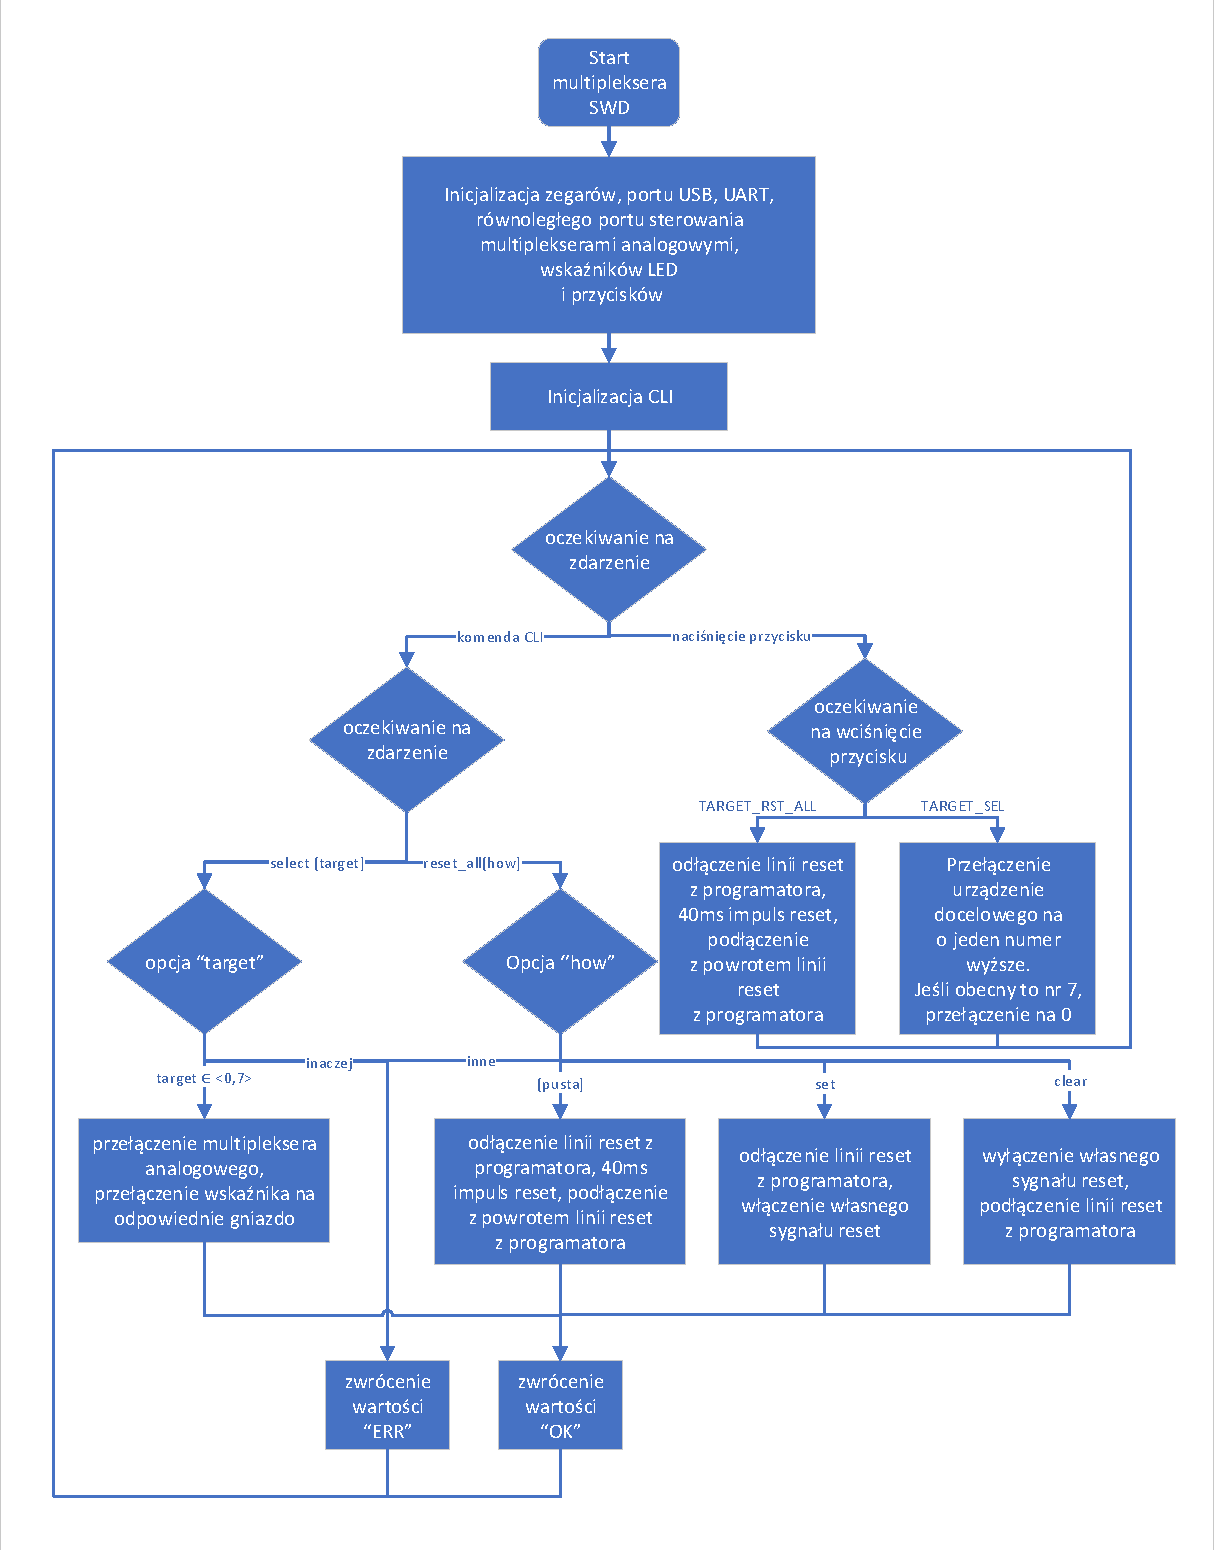
\includegraphics[width=0.72\paperwidth]{images/Mux_blokowy_soft.pdf}
\caption{Schemat blokowy oprogramowania układowego multipleksera SWD}
\label{SWD_MUX_software_block_diagram}
\end{figure}
\end{center}



\section {Oprogramowanie PC}
Multiplekser SWD jest urządzeniem, które wykorzystywane jest na etapie rozwoju i testów oprogramowania wbudowanego. Z racji dużej popularności interpretera Python w tej dziedzinie, najwygodniejsze jest użycie właśnie tego języka do wydawania prostych poleceń przez port szeregowy. Ponadto czyni to program łatwo przenośnym pomiędzy różnymi systemami operacyjnymi po drobnych modyfikacjach wynikających np. z różnicy komend używanych w różnych systemach operacyjnych.

Wymagania oprogramowania to:
\begin{enumerate}
    \item System operacyjny Microsoft Windows
    \item Interpreter Python 3
    \item oprogramowanie J-Link Commander (od wersji v6.60, dodatkowo wymagane dodanie folderu  \emph{bin} z katalogu instalacyjnego oprogramowania J-Linka do zmiennej środowiskowej PATH w systemie operacyjnym)
\end{enumerate}


Oprogramowanie na PC spełnia 3  główne funkcje:
\begin{enumerate}
    \item Zmiana urządzenia docelowego. Program sprawdza, czy bieżące urządzenie jest inne niż wybrane. Jeśli tak, wysyłana jest komenda do multipleksera SWD. Jeśli bieżące urządzenie jest w stanie resetu indywidualnego, jest on wyłączany.
    \item Resetowanie wszystkich urządzeń jednocześnie. Polega na wysłaniu komendy \emph{reset\_all} z opcją podaną w argumencie. Domyślnie nie ma opcji.
    \item Resetowanie bieżącego urządzenia. Realizowane przez skrypt uruchamiany w J-Link Commander. Funkcja przyjmuje argument analogicznie do funkcji \emph{reset\_all}
    \item Przesyłanie oprogramowania do urządzenia docelowego. Funkcja tworzy i uruchamia skrypt w J-Link Commander. Obsługiwany format pliku to ".hex".
\end{enumerate}

Biblioteka napisana jest w taki sposób, aby każdemu urządzeniu docelowemu można było zdefiniować inny plik zawierający jego oprogramowanie. Ponadto przewiduje możliwość programowania różnych modeli urządzeń. 



